%%%%%%%%%%%%%%%%%%%%%%%%%%%%%%% beamer %%%%%%%%%%%%%%%%%%%%%%%%%%%%%%%%%%%%%%%%%%%%%%%%%
% To run - pdflatex filename.tex
%      acroread filename.pdf
%%%%%%%%%%%%%%%%%%%%%%%%%%%%%%%%%%%%%%%%%%%%%%%%%%%%%%%%%%%%%%%%%%%%%%%%%%%%%%%%%%%%%%%%

\documentclass[compress,oilve]{beamer}
\mode<presentation>

\usetheme[]{CambridgeUS}
% other themes: AnnArbor, Antibes, Bergen, Berkeley, Berlin, Boadilla, boxes, CambridgeUS, Copenhagen, Darmstadt, default, Dresden, Frankfurt, Goettingen,
% Hannover, Ilmenau, JuanLesPins, Luebeck, Madrid, Maloe, Marburg, Montpellier, PaloAlto, Pittsburg, Rochester, Singapore, Szeged, classic

\usecolortheme{beaver}
% color themes: albatross, beaver, beetle, crane, default, dolphin,  fly, lily, orchid, rose, seagull, seahorse, sidebartab, whale, wolverine

\usefonttheme{professionalfonts}
% font themes: default, professionalfonts, serif, structurebold, structureitalicserif, structuresmallcapsserif


\hypersetup{pdfpagemode=FullScreen} % makes your presentation go automatically to full screen

% define your own colors:
\definecolor{Red}{rgb}{1,0,0}
\definecolor{Blue}{rgb}{0,0,1}
\definecolor{Green}{rgb}{0,1,0}
\definecolor{magenta}{rgb}{1,0,.6}
\definecolor{lightblue}{rgb}{0,.5,1}
\definecolor{lightpurple}{rgb}{0.8, 0.6, 0.9}
\definecolor{gold}{rgb}{.6,.5,0}
\definecolor{orange}{rgb}{1,0.4,0}
\definecolor{hotpink}{rgb}{1,0,0.5}
\definecolor{newcolor2}{rgb}{.5,.3,.5}
\definecolor{newcolor}{rgb}{0,.3,1}
\definecolor{newcolor3}{rgb}{1,0,.35}
\definecolor{darkgreen1}{rgb}{0, .35, 0}
\definecolor{darkgreen}{rgb}{0, .6, 0}
\definecolor{darkred}{rgb}{.75,0,0}
\definecolor{skyblue}{HTML}{75bbfd}

\definecolor{olive}{cmyk}{0.64,0,0.95,0.4}
\definecolor{purpleish}{cmyk}{0.75,0.75,0,0}

% can also choose different themes for the "inside" and "outside"

% \usepackage{beamerinnertheme_______}
% inner themes include circles, default, inmargin, rectangles, rounded

% \usepackage{beamerouterthemesmoothbars}
% outer themes include default, infolines, miniframes, shadow, sidebar, smoothbars, smoothtree, split, tree


\useoutertheme[subsection=true, height=40pt]{smoothbars}

% to have the same footer on all slides
%\setbeamertemplate{footline}[text line]{STUFF HERE!}
\setbeamertemplate{footline}[text line]{} % makes the footer EMPTY
% include packages
%

%show the page numbers in footnote
%\addtobeamertemplate{navigation symbols}{}{%
%	\usebeamerfont{footline}%
%	\usebeamercolor[fg]{footline}%
%	\hspace{1em}%
%	\insertframenumber/\inserttotalframenumber
%}

\setbeamercolor{footline}{fg=purpleish}
\setbeamerfont{footline}{series=\bfseries}

%add color to curent subsection
\setbeamertemplate{section in head/foot}{\hfill\tikz\node[rectangle, fill=darkred, rounded corners=1pt,inner sep=1pt,] {\textcolor{white}{\insertsectionhead}};}
\setbeamertemplate{section in head/foot shaded}{\textcolor{darkred}{\hfill\insertsectionhead}}

% Remove bullet of subsections
\setbeamertemplate{headline}
{%
	\begin{beamercolorbox}{section in head/foot}
		\insertsectionnavigationhorizontal{\textwidth}{}{}
	\end{beamercolorbox}%
}


% modify headlline, specially headline size
\setbeamertemplate{headline}{%
	\leavevmode%
	\hbox{%
		\begin{beamercolorbox}[wd=\paperwidth,ht=3.5ex,dp=1.125ex]{palette quaternary}%
			\insertsectionnavigationhorizontal{\paperwidth}{}{\hskip0pt plus1filll}
		\end{beamercolorbox}%
	}
}

\setbeamertemplate{footline}{%
	\leavevmode%
	\hbox{\begin{beamercolorbox}[wd=.5\paperwidth,ht=2.5ex,dp=1.125ex,leftskip=.3cm plus1fill,rightskip=.3cm]{author in head/foot}%
			\usebeamerfont{author in head/foot}\insertshortauthor ~ \insertshortinstitute
		\end{beamercolorbox}%
		\begin{beamercolorbox}[wd=.5\paperwidth,ht=2.5ex,dp=1.125ex,leftskip=.3cm,rightskip=.3cm plus1fil]{title in head/foot}%
			\usebeamerfont{title in head/foot}\insertshorttitle\hfill\insertframenumber\,/\,\inserttotalframenumber
	\end{beamercolorbox}}%
	\vskip0pt%
}


%\setbeamertemplate{navigation symbols}{}

\title{Unsupervised Learning: Dimensionality Reduction}
\author{ML Instruction Team, Fall 2022}
\institute[]{CE Department \newline  Sharif University of Technology \newline \newline}
\date[\today]{}
%\titlegraphic{\includegraphics[scale=.35]{example-image}}



%Write \usepackage{etex} just after the \documentclass line (it should be the first loaded package).
\usepackage{etex}
\usepackage{subcaption}
\usepackage{multicol}
\usepackage{physics, amsmath}
\usepackage{epsfig}
\usepackage{graphicx}
\usepackage{amsfonts}
\usepackage{amssymb}
\usepackage[all,knot]{xy}
\xyoption{arc}
\usepackage{url}
\usepackage{multimedia}
\usepackage{hyperref}
\hypersetup{colorlinks,linkcolor=blue,citecolor=redorange,urlcolor=darkred}
\usepackage{multirow}
\usepackage[font={scriptsize}]{caption}
\usepackage{pgf}
\usepackage{fontspec}
\usepackage{subcaption}
\usepackage[export]{adjustbox}
\usepackage{caption}
%\setsansfont[Scale=MatchLowercase, BoldFont = * Bold, ItalicFont = * Italic]{Caladea}
\graphicspath{ {./Pictures/} }
%\usepackage{enumitem,xcolor}
%\newcommand{\labelitemi}{$\blacksquare$}
%\newcommand{\labelitemii}{$\diamond$}
%\newcommand{\labelitemiii}{$\square$}
%\newcommand{\labelitemiv}{$\ast$}
%\setbeamercolor*{item}{fg=red}
\usepackage{bm}
\usepackage{xcolor}
\usepackage[backend=biber]{biblatex}
\definecolor{keywords}{rgb}{.224,.451,.686}

\newcommand{\tc}[2]{
 \textcolor{#1}{\textbf{#2}}
}


\usefonttheme{professionalfonts} 
\setbeamertemplate{itemize item}{\color{skyblue}$\blacksquare$}
\setbeamertemplate{itemize subitem}{\color{hotpink}$\blacktriangleright$}
\setbeamertemplate{itemize subsubitem}{\color{orange}$\bullet$}


\usepackage{anyfontsize}
\usepackage{t1enc}
\usepackage{tikz}
\usetikzlibrary{calc,trees,positioning,arrows,chains,shapes.geometric,decorations.pathreplacing,decorations.pathmorphing,shapes,matrix,shapes.symbols}


\DeclareMathOperator*{\argmin}{argmin}
\newtheorem{proposition}[theorem]{Proposition}
\newtheorem{remark}[theorem]{Remark}
\newtheorem{assumption}[theorem]{Assumption}

\usepackage{fontspec,unicode-math}
\setmainfont[Scale=0.9]{Consolas}
\setmonofont[Scale=0.9]{Monaco}
\setsansfont[Scale=1]{Times New Roman}
\newcommand{\vect}[1]{\boldsymbol{#1}}


%\usepackage{smartdiagram}
%\usesmartdiagramlibrary{additions}
%%%%%%%%%%%%%%%%%%%%%%%%%%%%%%%%%%%%%%%%%%%%%%%%%%%%%%%%%%%%%%%%%%%%%%%%%%%%%%%%%%%%%%%%%%%%
%%%%%%%%%%%%%%%%%%%%%%%%%%%%%% Title Page Info %%%%%%%%%%%%%%%%%%%%%%%%%%%%%%%%%%%%%%%%%%%
%%%%%%%%%%%%%%%%%%%%%%%%%%%%%%%%%%%%%%%%%%%%%%%%%%%%%%%%%%%%%%%%%%%%%%%%%%%%%%%%%%%%%%%%%%


%%%%%%%%%%%%%%%%%%%%%%%%%%%%%%%%%%%%%%%%%%%%%%%%%%%%%%%%%%%%%%%%%%%%%%%%%%%%%%%%%%%%%%%%%%
%%%%%%%%%%%%%%%%%%%%%%%%%%%%%% Begin Your Document %%%%%%%%%%%%%%%%%%%%%%%%%%%%%%%%%%%%%%%
%%%%%%%%%%%%%%%%%%%%%%%%%%%%%%%%%%%%%%%%%%%%%%%%%%%%%%%%%%%%%%%%%%%%%%%%%%%%%%%%%%%%%%%%%%
\begin{document}
	
%%%%%%%%%%%%%%%%%%%%%%%%%%%%%%%%%%%%%%%%%%%%%%%%%%%%%%%%%%%%%%%%%%%%%%%%%%%%%%%%%%%%%%%%%%
	\fontsize{9}{9}
\begin{frame}[noframenumbering, plain]
	\titlepage
\end{frame}

%%%%%%%%%%%%%%%%%%%%%%%%%%%%%%%%%%%%%%%%%%%%%%%%%%%%%%%%%%%%%%%%%%%%%%%%%%%%%%%%%%%%%%%%%%
\section{Dimensionality Reduction: An Overview}
%%%%%%%%%%%%%%%%%%%%%%%%%%%%%%%%%%%%%%%%%%%%%%%%%%%%%%%%%%%%%%%%%%%%%%%%######

%%%%%%%%%%%%%%%%%%%%%%%%%%%%%%%%%%%%%%%%%%%%%%%%%%%%%%%%
\begin{frame}{Dimensionality Reduction: An Overview}
\begin{itemize}
\item \tc{keywords}{Why Dimensionality Reduction ?}
	\medskip
\item Consider a data set that contains image of letter A which has been scaled and rotated. each image of A is a $ 32 \times 32 $ pixel image so it would be a 1024 dimensional data.

\end{itemize}
\begin{figure}
		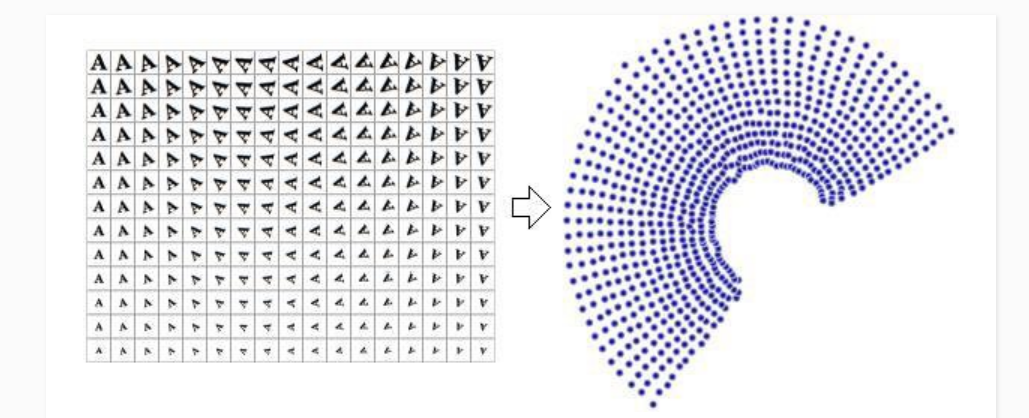
\includegraphics[scale=0.5]{3}
		\caption{Dimensionality Reduction, \href{https://tinyurl.com/2q6ec2c6}{Source}}
	\end{figure}
%\begin{figure}[htbp!]
%		\subfloat[][Dimensionality Reduction, \href{https://tinyurl.com/2graetht}{Source}]
	%	{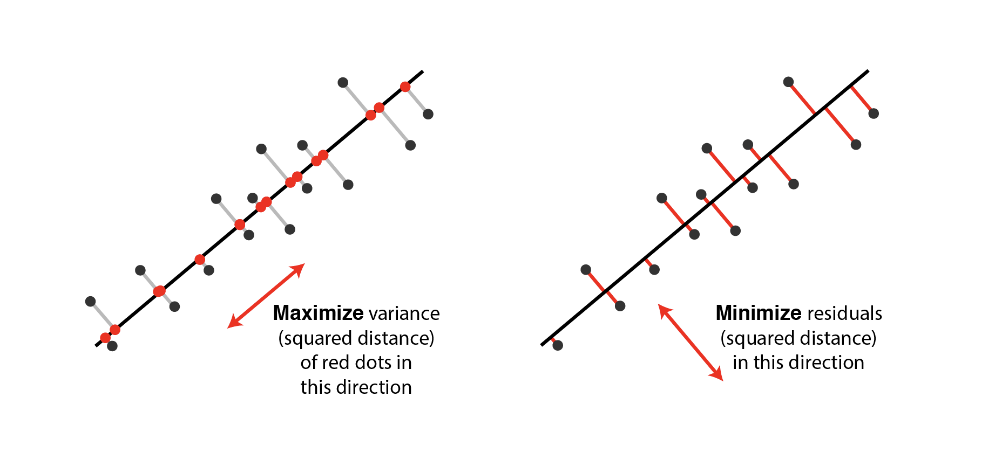
\includegraphics[scale=0.5]{1}
	%		\label{fig:subfigure1}}
	%	\qquad
	%	\subfloat[][Dimensionality Reduction, \href{https://tinyurl.com/2n32ohqf}{Source}]
	%	{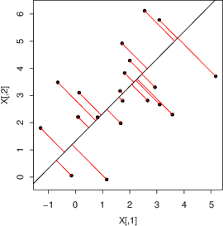
\includegraphics[scale=0.5]{2}
	%		\label{fig:subfigure2}}
	%	\\
		
	%	\tiny
	%	\caption{Different clustering techniques}
	%	\label{fig:globalfigure2}
		
	%\end{figure}
\end{frame}

\begin{frame}{Dimensionality Reduction: An Overview}
\begin{itemize}
\item However, in the preceding picture, it looks like that the actual dimension of the data is two because only two variables namely rotation and scale used to generate the data set.
\medskip
\item A successful dimensionality reduction progress would extract the variable information (rotation and scale) and discard the correlated information (letter A)
\medskip
\item Unlike clustering, which we searched for the discerte latent variables, such as number of clusters and the behavior of them, in dimensionality reduction we would like to find the \tc{keywords}{continuous latent variables}. these important features are also called \tc{keywords}{degrees of freedom}.
\medskip
\item In general, we would like to discover another data space which has much lower dimensionality than the original data space and these data are closed to it.
\end{itemize}
\end{frame}


\section{An Overview of PCA}
\begin{frame}{An Overview of PCA}
\begin{itemize}
\item One of the most widely used techniques in order to do the dimensionality reduction is \tc{keywords}{Principal Compponent Analysis} or \tc{keywords}{PCA}.
\item Principal Component Analysis is usually defined in two ways, although these two definitions are eqauivalent:
\begin{itemize}
\item \tc{keywords}{Maximum Variance Formulation}
\item \tc{keywords}{Minimum Error Formulation}
\end{itemize}
\end{itemize}
\begin{figure}
		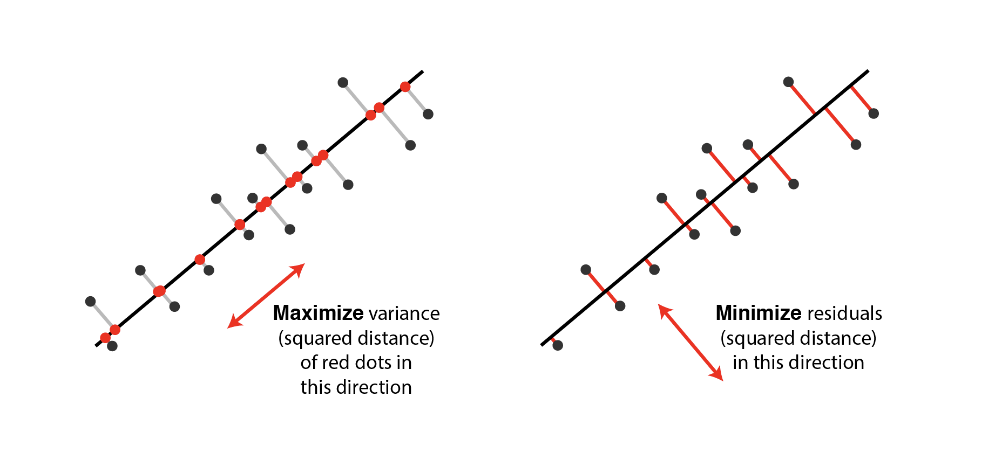
\includegraphics[scale=0.5]{1}
		\caption{Illustration of PCA, \href{	https://tinyurl.com/2q6ec2c6}{Source}}
	\end{figure}
\end{frame}




\section{PCA in Detail: Maximum Variance Formulation}
\begin{frame}{PCA in Detail: Maximum Variance Formulation}
\begin{itemize}
\item Consider we have a $ D $ dimensional data set $\{ \mathbf{x_{\mathnormal n}}  \}$, which we would like to reduce the number of dimensions to  the $M  (M < D) $ . without loss of generality we assume that the $ M = 1 $. we then generalize the case of $M$-dimensional by induction.
\medskip
\item We would like to compute the variance of projected data and then maximize it, if we assume that the direction of real line in $D$-dimensional space is shown by a unit vector called $\mathbf{u_{1}}$, then the emprical covariance of projected 1-Dimensoional data would be:



\begin{equation}
\begin{aligned}	
Cov = \frac{1}{N - 1} \displaystyle\sum_{n=1}^{N} \big( \mathbf{u_{1}}^{T} \mathbf{x_{\mathnormal n}} - \mathbf{u_{1}}^{T } \mathbf{\bar{x}} \big) ^ {2} = \mathbf{u_{1}}^{T} \mathbf{S} \mathbf{u_{1}}\\ \text{where} \quad \mathbf{\bar{x}} =  \frac{1}{N} \displaystyle\sum_{n=1}^{N} \mathbf{x_{\mathnormal n}} \quad \text{,} \quad \mathbf{S} = \frac{1}{N-1} \displaystyle\sum_{n=1}^{N} \big( \mathbf{x_{\mathnormal n}}  -   \mathbf{\bar{x}} \big)  \big( \mathbf{x_{\mathnormal n}}  -   \mathbf{\bar{x}} \big) ^ {T} 
\end{aligned}
\end{equation}

\end{itemize}
\end{frame}



\begin{frame}{PCA in Detail: Maximum Variance Formulation}
\begin{itemize}
\item In order to maximize the variance we would have a constrainted optimization problem like this:
\begin{equation}
\begin{aligned}
\max_{\mathbf{u_{1}}} \quad & \mathbf{u_{1}}^{T} \mathbf{S}\mathbf{u_{1}}\\
\textrm{subject to} \quad & 1 - \mathbf{u_{1}}^{T}\mathbf{u_{1}} = 0\\
\end{aligned}
\end{equation}
\item If we use the Lagrangian multiplier we have an unconstrainted optimization:
\begin{equation}
\begin{aligned}
\max_{\mathbf{u_{1}}} \quad & \mathbf{u_{1}}^{T} \mathbf{S}\mathbf{u_{1}} + \lambda_{1}(1 - \mathbf{u_{1}}^{T}\mathbf{u_{1}})\\
\end{aligned}
\end{equation}
\item Taking deravitive of preceding term respect to $\mathbf{u_{1}}$ and set it to zero would give us:
\begin{equation}
\begin{aligned}
\mathbf{S} \mathbf{u_{1}} = \lambda_{1}\mathbf{u_{1}}
\end{aligned}
\end{equation}

\item It is obvious that the $ \mathbf{u_{1}} $ must be the \tc{keywords}{eigenvector} of $ \mathbf{S} $ and the $ \lambda_{1}$ is the corresponding \tc{keywords}{eigenvalue} , this eigenvector is known as \tc{keywords}{first principal component}. if we left-multiply both side of above equation by $\mathbf{u_{1}}^{T}$, the maximum variance is given by:
\begin{equation}
\begin{aligned}
\mathbf{u_{1}}^{T}\mathbf{S} \mathbf{u_{1}} = \lambda_{1}
\end{aligned}
\end{equation}
\end{itemize}



\end{frame}





\begin{frame}{PCA in Detail: Singular Value Decomposition}
\begin{itemize}
\item As a result, we must take the $\mathbf{u_{1}}$ which has the \tc{keywords}{largest} $\lambda_{1} $ value corresponding to it.
\item We can consider the general $M$-dimensional case by obtaining $ \mathbf{u_{1}}, \mathbf{u_{2}}, \dots, \mathbf{u_{m}} $ corresponding to the first $M$ large eigenvalues $  \lambda_{1},  \lambda_{2}, \dots, \lambda_{m} $. this can easily shown by induction
\item To summerize, PCA is dealing with the covariance matrix of the data set and searching for $M$ largest eigenvalues corresponding to the $M$ eigenvectors that form the basis of the final subspace.
\end{itemize}
\begin{figure}
		\centering
		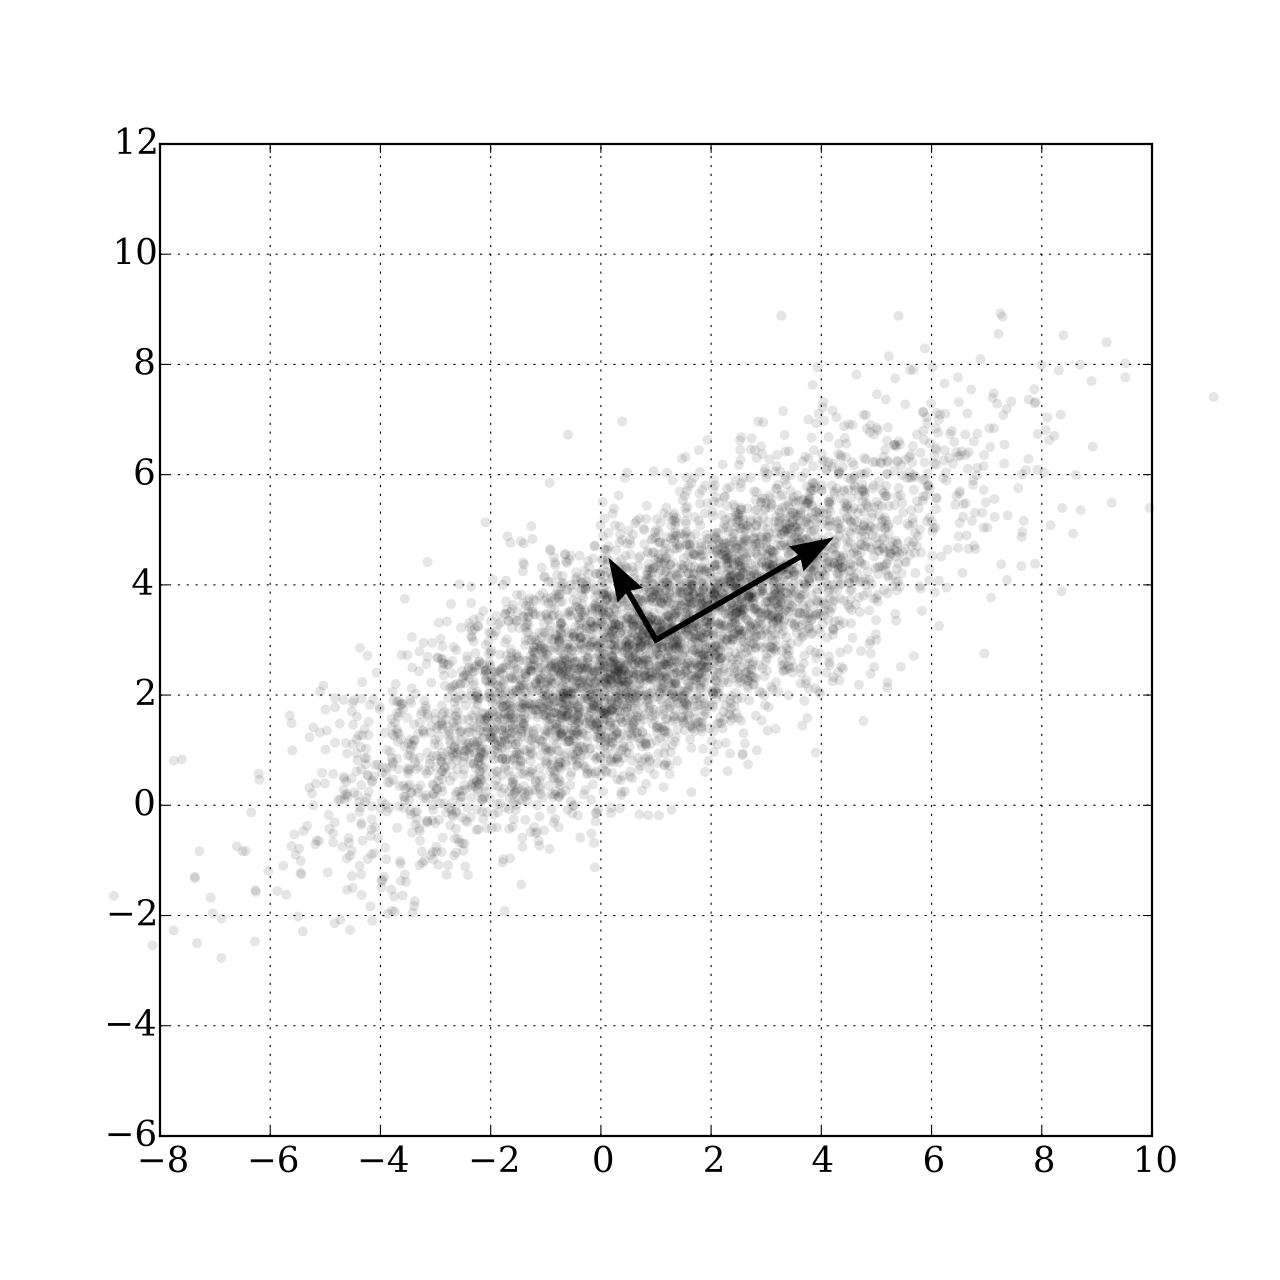
\includegraphics[scale=0.1]{5}
		\caption{Illustration of PCA, \href{	https://tinyurl.com/2q6ec2c6}{Source}}
	\end{figure}


\end{frame}
%%%%%%%%%%%%%%%%%%%%%%%%%%%%%% %

\begin{frame}{PCA in Detail: Singular Value Decomposition}
\begin{itemize}
\item There are several techniques to decompose the eigenvectors, but the most useful solution is \tc{keywords}{Singular Value Decomposition}.
\end{itemize}
\begin{figure}
		\centering
		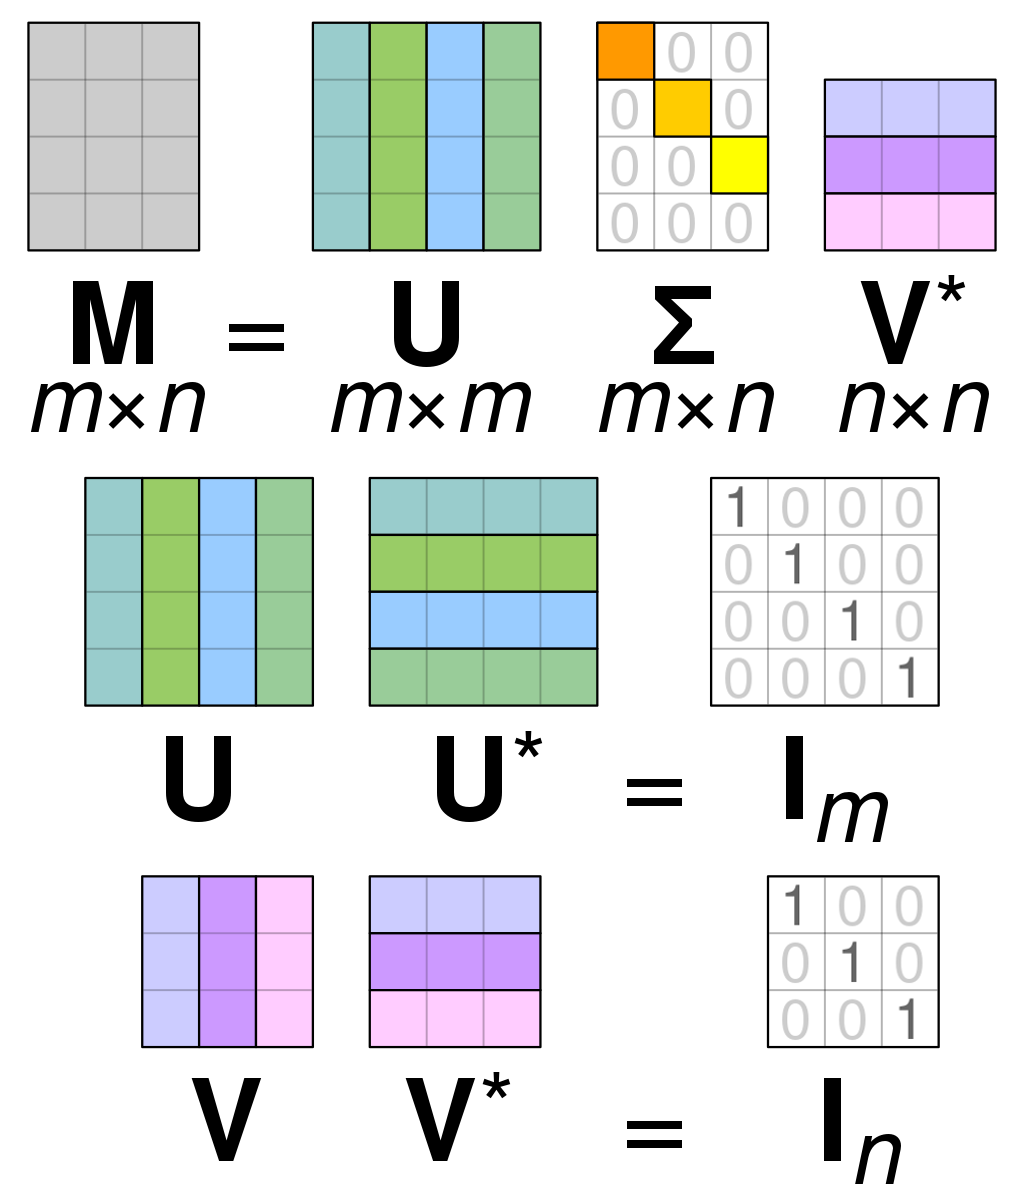
\includegraphics[scale=0.1]{4}
		\caption{Illustration of SVD, \href{	https://tinyurl.com/2q6ec2c6}{Source}}
	\end{figure}


\end{frame}




\frametitle{Final Notes}
\centering
\vspace{50 pt}
\textbf{Thank You!}
\vspace{50pt}

\textbf{Any Question?}
%%%%%%%%%%%%%%%%%%%%%%%%%%%%%%%%%%%%%%%%%%
\end{document}